\documentclass[output=paper,modfonts,newtxmath,hidelinks]{langscibook} 
\ChapterDOI{10.5281/zenodo.2545533}


\title{Gender encoding on hybrid nouns in Bosnian\slash Croatian\slash Serbian:\newlineCover Experimental evidence from ellipsis} 

\author{Andrew Murphy\affiliation{University of Leipzig}\and  Zorica Puškar\affiliation{Leibniz-Zentrum Allgemeine Sprachwissenschaft, Berlin}\lastand  Matías Guzmán Naranjo\affiliation{Heinrich Heine University Düsseldorf}}

\abstract{In this paper, we report the results of an experimental study on the possibility of gender mismatches with ellipsis of a particular type of hybrid nouns  in Bosnian / Croatian / Serbian (henceforth: BCS).    Using agreement mismatches under NP ellipsis as a diagnostic for gender feature specification of hybrid nouns, we show  that these nouns disallow agreement mismatches under NP ellipsis if natural gender (and a presupposition that it introduces) is present either in the antecedent or the ellipsis site.   We argue that natural gender feature (masculine in our study)  can optionally be present on the hybrid noun, and that its inclusion in ellipsis contexts leads to a violation of the standard identity requirement between the antecedent and the ellipsis site, namely \citeauthor{merchant2001}'s (\citeyear{merchant2001}) e-\textsc{given}ness.
 
\keywords{gender features, ellipsis, agreement, mismatches}
}

\begin{document}
\maketitle
\shorttitlerunninghead{Gender encoding on hybrid nouns in Bosnian/Croatian/Serbian}

\section{Introduction: Hybrid nouns in BCS}

Hybrid nouns have been a challenge for theories of agreement and NP structure (see \citealt{corbett91,wandz03,aandalfg,aandalanguage,pesetsky14,kramerbook,Landau2016DPinternalsemantic,smith15,smith16,arsenijevicjuksek,despichybrid17}), as it seems that they can simultaneously bear two types of gender specification: 
(i) natural gender (reflecting the gender of the referent) and
(ii) grammatical gender (assigned arbitrarily). In this paper, we focus only on the Class II hybrid nouns in BCS (ending in \textit{-a}) which have grammatical feminine gender, but variable natural gender, which depends on the discourse referent.
	

\begin{table}
\caption{Some hybrid nouns in BCS}\label{14:t1}
% \hspace*{-0.2em}\resizebox{.94\textwidth}{!}{
\small
\begin{tabularx}{\textwidth}{llllll}
\lsptoprule
% \multicolumn{2}{c}{\textit{-a}} & \multicolumn{2}{c}{\textit{-ica}} & \multicolumn{2}{c}{\textit{-(č)ina}} \\
\textbf{\textit{-a}}&&\textbf{\textit{-ica}}&&\textbf{\textit{-(č)ina}}&\\
\midrule
\textit{mušterija} & `customer' &  \textit{varalica} & `cheater'  & \textit{junačina} & `great hero'\\  
\textit{budala} & `fool'  & \textit{propalica} & `loser, failure' & \textit{dobričina} & `very good person'\\
\textit{sudija} & `judge' & \textit{pijanica} & `drunkard'  & \textit{drugarčina} & `a great friend'\\
\textit{tužibaba} & `telltale' & \textit{spavalica} & `sleeper' & \textit{lažovčina} & `a big liar' \\
\lspbottomrule
\end{tabularx}
\end{table}
% }
% \vspace*{0.5em}	

\noindent For instance, with a masculine referent, the noun \textit{mušterija} (`customer') can trigger either grammatical feminine  \REF{14:ex1a}/\REF{14:ex1b} or natural masculine agreement  \REF{14:ex1c}/\REF{14:ex1d} (subject to speaker variability).
	
	\ea \label{14:ex1}
	\ea[]{\gll Milan nam je nov-a mušterija.\\
	Milan us is new-\textsc{f} customer\\
	\glt `Milan is our new customer.'}\label{14:ex1a}
	\ex[]{\gll Nov-a mušterija je kupila jaknu.\\
	new-\textsc{f} customer is bought.\textsc{f} jacket.\\
	\glt `A new (male or female) customer bought a jacket.'}\label{14:ex1b}
	\ex[\%]{\gll Milan nam je nov-i mušterija.\\
	Milan us is new-\textsc{m} customer\\
	\glt `Milan is our new customer.'}\label{14:ex1c}
	\ex[\%]{\gll Nov-i mušterija je kupio jaknu.\\
	new-\textsc{m} customer is bought.\textsc{m} jacket.\\
	\glt `A new (male) customer bought a jacket.'}\label{14:ex1d}
    \z \z
	
\noindent With female referents, however, such nouns can only trigger feminine agreement:
	
	\ea \label{14:ex2}
	\gll Marija nam je nov-a / *\hspace{-2pt} nov-i mušterija.\\
	Marija us is new-\textsc{f} {} {} new-\textsc{m} customer\\
     \glt `Marija is our new customer.'
 \z
		
\noindent One could treat these as so-called ``epicene'' nouns of the type found e.g. in Brazilian Portuguese and Greek, which can be used with both masculine and feminine referents without change in form \citep{bobaljikzocca,merchant14,kramerbook}.
 It has been proposed that such nouns are simply listed in the lexicon twice, each with a different gender feature \citep[e.g.][19]{merchant14}. However, such an approach to BCS hybrid nouns seems to be problematic, as there is evidence that these nouns can \textit{simultaneously} bear natural and grammatical gender. 
 For example, in \REF{14:ex3} the adjective and determiner target different gender values of the noun, while \REF{14:ex4} shows the same for the nominal modifier and the participle.\footnote{Relative pronouns can also show different gender values than the attributive modifiers of a hybrid noun, as shown in \REF{14:exfn1i}, obtained at \url{http://vukajlija.com/seoski-fudbalski-tim-iz-beton-lige} $<$accessed 26.11.2016$>$.
 
\ea \gll Lokaln-a pijanica, koj-i je završio sa igranjem fudbala...\\
	local-\fbox{\textsc{f.sg}} drunkard, who-\fbox{\textsc{m.sg}} is finished.\textsc{m.sg} with playing football\\
	\glt `A local drunkard, who's finished playing football...'\label{14:exfn1i}
    \z

\noindent However, as pointed out by a reviewer, whether the relative pronoun agrees directly with the hybrid noun, or whether agreement is more indirect (since we are dealing with a non-restrictive relative clause in which the relative pronoun is more akin to regular pronouns, c.f. \citealt{devries06}) is an issue that requires further investigation. See \citet{arsenijevicjuksek} for further discussion on hybrid agreement with relative pronouns.}	

	\ea \gll ov-i privatn-e zanatlije\label{14:mismatchbcs}\\
	these-\fbox{\textsc{m.pl}} private-\fbox{\textsc{f.pl}} artisan.\textsc{pl}\\
	\glt `these private artisans'\hfill \citep[206]{corbett06}\label{14:ex3}
    \z
	
	\ea \gll Osm-a budala je bio-$\emptyset$ mnogo kul tip ali su ga se drugi malo plašili.\footnotemark\\
	eighth-\fbox{\textsc{f.sg}} fool.\textsc{sg} is been-\fbox{\textsc{m.sg}} very cool guy but are him \textsc{refl} others little feared\\
	\glt `The eighth fool was a very cool guy, but others were a bit afraid of him.'\label{14:ex4}
    \z
 
 \footnotetext{\url{http://magdajanjic.tumblr.com/post/85348961537/budala} $<$accessed 26.11.2016$>$.}
	
	
	

\noindent These examples raise the question about the structural representation of such nouns: whether they do contain both types of gender feature simultaneously, and how exatly they should be represented. In what follows, we will answer these questions by using NP ellipsis as a diagnostic for the gender feature specification of BCS hybrid nouns.

\section{Gender mismatches and NP ellipsis}

There is a growing body of literature on the permissibility of gender mismatches under NP ellipsis  \citep[e.g.][]{nuneszocca10,bobaljikzocca,merchant14,sudospathas-sub20,barrie-cayuga16}.
Based on whether gender mismatches under NP ellipsis are allowed or not, previous literature has identified three classes of nouns. The first type are the \textsc{two-way alternating nouns} (henceforth: the \textit{doctor}-class), where a masculine antecedent can license deletion of a noun with a feminine referent, and \textit{vice versa:}

\ea \textbf{Two-way alternating nouns} (\textit{doctor}-class)\label{14:ex5}
\ea \gll O Petros ine kalos jatros, ala i Maria ine mia kakia $\langle$jatros$\rangle$.\\	 
	 the Petros is good.\textsc{m} doctor but the Maria is a.\textsc{f} bad.\textsc{f} ~doctor\\
	 \glt `Petros is a good doctor, but Maria is a bad one.'
\ex \gll I Maria ine kali jatros, ala o Petros ine enas kakos $\langle$jatros$\rangle$.\\ 	 
	 the Maria is good.\textsc{f} doctor but the Petros is a.\textsc{m} bad.\textsc{m} ~doctor\\
	 \glt `Maria is a good doctor, but Petros is a bad one.'	\\ \hspace*\fill (Greek; \citealt[15]{merchant14})
     \z \z
     
     
\noindent The second type are the \textsc{non-alternating nouns} (henceforth: \textit{brother}-class), which do not allow mismatches in either direction:
	 
\ea \textbf{Non-alternating nouns} (\textit{brother}-class)
\ea[*]{\gll O Petros ine kalos adherfos, ala i Maria ine mia kakia $\langle$adherfi$\rangle$.\\
	the Petros is good.\textsc{m} brother but the Maria is a.\textsc{f} bad.\textsc{f} ~sister\\
	\glt Intended: `Petros is a good brother, but Maria is a bad one (sister).'}
\ex[*]{\gll I Maria ine kali adherfi, ala o Petros ine enes kakos $\langle$adherfos$\rangle$.\\
	the Maria is good.\textsc{f} sister but the Petros is a.\textsc{m} bad.\textsc{m} ~brother\\
	\glt Intended: `Petros is a good brother, but Maria is a bad one (sister).'	 \\ \hspace*\fill (Greek; \citealt[12]{merchant14})}
    \z \z
	 
\noindent Finally, \textsc{one-way alternating nouns}  (or the \textit{actor}-class) allow a masculine noun to antecede an elided feminine noun \REF{14:ex7a}, but a mismatch in the opposite direction is ungrammatical \REF{14:ex7b}.

% \newpage
\ea  \textbf{One-way alternating nouns} (\textit{actor}-class)
\ea[?]{\gll O Paulo é ator e a Fernanda também é $\langle$\hspace{-2pt} atriz$\rangle$.\\
	 the Paulo is actor and the Fernanda also is {} actress\\
	 \glt `Paulo is an actor and Fernanda is too.'}\label{14:ex7a}
\ex[*]{\gll A Fernanda é atriz e o Paulo também é $\langle$\hspace{-2pt} ator$\rangle$.\\
     the Fernanda is actress and the Paulo also is {} actor\\
	 \glt Intended: `Fernanda is an actress and Paulo is (an actor) too.'\label{14:ex7b}\\ \hspace*\fill (Brazilian Portuguese; \citealt[142]{bobaljikzocca})}
     \z \z

\noindent With regard to their tolerance for gender mismatches, these three classes can be summarized as in \tabref{14:t2}:     
     
     \begin{table}
     \caption{Classes of predicative nouns under ellipsis \citep[cf.][162]{bobaljikzocca}} \label{14:t2}
%    \hspace*{-0.2em}\resizebox{.94\textwidth}{!}{
\begin{tabularx}{\textwidth}{rccl}
\lsptoprule
\multicolumn{1}{c}{\multirow{2}{*}{\textbf{Class}}}	& \textbf{\textsc{masc} antecedent} 	&  	\textbf{\textsc{fem} antecedent} & \multicolumn{1}{c}{\multirow{2}{*}{\textbf{Type}}}\\
						& \textbf{\textsc{fem} ellipsis} 	& 	\textbf{\textsc{masc} ellipsis} & \\
\midrule
\textit{doctor}-class & {\ding{51}} & {\ding{51}} & Two-way alternating\\
\textit{brother}-class & \ding{55} & \ding{55} & Non-alternating\\
\textit{actor}-class & {\ding{51}} & \ding{55} & One-way alternating\\
\lspbottomrule
\end{tabularx}
% }
\end{table}
% \vspace*{0.5em}
     
\noindent We would expect that hybrid nouns in BCS pattern with one of these types. However, the additional complication with hybrid nouns is that there is evidence for the simultaneous presence of two gender features.
Thus, we will try to gain some insight into their structure by testing the acceptability of gender mismatches with mismatched referents in either direction \REF{14:ex8b}/\REF{14:ex8c}.

\ea
  		\ea[]{\gll Milan mu je star-\textbf{a} mušterija, a Marija mu je nov-\textbf{a} $\langle$\hspace{-2pt} mušt.$\rangle$.\\
  		Milan him is old-\fbox{\textsc{f}} customer and Marija him is new-\fbox{\textsc{f}} {} cust.\\
  		\glt `Milan is his old customer and Marija a new one.'}
  		\ex[?]{\gll Milan mu je star-\textbf{i} mušterija, a Marija mu je nov-\textbf{a} $\langle$\hspace{-2pt} mušt.$\rangle$.\\
  		Milan him is old-\fbox{\textsc{m}} customer and Marija him is new-\fbox{\textsc{f}} {} cust.\\ 
  	\glt `Milan is his old customer and Marija a new one.' }\label{14:ex8b}
  		\ex[?]{\gll Marija mu je star-\textbf{a} mušterija, a Milan mu je nov-\textbf{i} $\langle$\hspace{-2pt} mušt.$\rangle$.\\
  		Marija him is old-\fbox{\textsc{f}} customer and Milan him is new-\fbox{\textsc{m}} {} cust.\\
  		\glt `Marija is his old customer and Milan a new one.'}\label{14:ex8c}
   \z \z
     
     
\section{Experiment}

The aim of the experiment was to discover whether an agreement mismatch was tolerated when masculine agreement was found either the antecedent \REF{14:ex8b} or the ellipsis site \REF{14:ex8c}, i.e. whether the hybrid nouns under study were two-way alternating, one-way alternating, or allowed no alternation at all when the noun had natural masculine gender  (indicated by the agreement on the adjective). Considering previous theories \citep{nuneszocca10,bobaljikzocca,merchant14,sudospathas-sub20}, the (im)possibility of a mismatch should be an indicator of (i) the difference in the quality of gender features (i.e. differences in ther semantics or morphosyntactic representation) and (ii) the licensing conditions on ellipsis (i.e. identity requirements between the antecedent and the ellipsis site). Finally, sentences in which both adjectives show feminine agreement, regardless of the gender of the subject, were expected to be grammatical, as the hybrid nouns in question have grammatical gender as a formal feature. 

In order to verify the grammaticality of gender mismatches under NP ellipsis, we ran an online acceptability judgement study.\footnote{For a detailed description of the design and for all the materials see \url{https://osf.io/r3npz}.} 
The experimental design involved the factors  in \REF{14:ex9}. The first factor involves the type of agreement the adjective has with a masculine subject and has two levels (grammatical agreement \textsc{mf} vs. natural agreement \textsc{mm}) \REF{14:ex9a}, which should serve as an indicator of the type of gender on the hybrid noun (grammatical vs. natural).
The second factor pertains to agreement with feminine subjects and has only a single level (\textsc{ff}, both grammatical and natural agreement) \REF{14:ex9b}. The final factor regards the position of the masculine referent and has two levels:
in the first clause, or in  the second clause (the one with NP ellipsis) \REF{14:ex9c}, which should indicate whether natural gender can function as an antecedent for ellipsis and whether it can be found in the ellipsis site. The $2\times 2\times 1$ combination of factors in \REF{14:ex9} yield the four experimental conditions in Table \ref{14:table:experimconditions}.

 \ea \textbf{Factors} (manipulated within items)\label{14:ex9}
  			\ea \textsc{agreement with masculine subject}; two levels: grammatical (\textsc{mf}) and natural (\textsc{mm})\label{14:ex9a}
  			\ex \textsc{agreement with feminine subject}; one level: \textsc{ff} \label{14:ex9b}
  			\ex \textsc{clause}; two levels: first and second\label{14:ex9c}
            \z \z
 
\begin{table}[h]
  		\centering
  		\begin{tabularx}{0.8\textwidth}{llp{2cm}llll}
		\lsptoprule
  			\multicolumn{4}{c}{\textbf{Factors and levels}} & & \textbf{Conditions}\\
%             \multirow{2}{*}{\textbf{Condition}}\\ 
			%\midrule
  			& \textsc{m.subj.agr}         & \textsc{clause} & \textsc{f.subj.agr}  &               & \\
			\midrule
  			1  & \textsc{mf}     & first  & \textsc{ff}          & ~~  & \textsc{mfff} \\
  			2  & \textsc{mm}     & first  & \textsc{ff}          &     & \textsc{mmff} \\	
  			3  & \textsc{mf}     & second & \textsc{ff}          &   & \textsc{ffmf} \\
  			4  & \textsc{mm}     & second & \textsc{ff}          &    &  \textsc{ffmm} \\\lspbottomrule
  		\end{tabularx}
  		\caption{\label{14:table:experimconditions}Experimental conditions}
  	\end{table}	

\noindent Some example test sentences for each condition are given below. Each contains two clauses coordinated by the conjunction \textit{a} `and' and an elided noun in the second conjunct. Sentences \REF{14:ex10} and \REF{14:ex12} were expected to be perceived as grammatical, while \REF{14:ex11} and \REF{14:ex13} were the relevant mismatching cases.
 
 
\ea \gll Jovan je redovn{-a} mušterija, a Milica povremen{-a} \underline{\hspace{1.5cm}}.\\
  		Jovan is regular{-\textsc{f}} customer and Milica occasional{-\textsc{f}}\\
  		\glt `Jovan is a regular customer and Milica an occasional one.'\hfill \textsc{mfff}\label{14:ex10}
        \z
  		
  		\ea \gll Jovan je redovn{-i} mušterija, a Milica povremen{-a} \underline{\hspace{1.5cm}}.\\
  		Jovan is regular{-\textsc{m}} customer and Milica occasional{-\textsc{f}}\\
  		\glt `Jovan is a regular customer and Milica an occasional one.'\hfill  \textsc{mmff}\label{14:ex11}
        \z
 
  		\ea \gll Milica je povremen{-a} mušterija, a Jovan redovn{-a} \underline{\hspace{1.5cm}}.\\
  		Milica is occasional{-\textsc{f}} customer and Jovan regular{-\textsc{f}}\\
  		\glt `Milica is an occasional customer and Jovan a regular one.'\hfill  \textsc{ffmf}\label{14:ex12}
        \z
  		
  		\ea \gll Milica je povremen{-a} mušterija, a Jovan redovn{-i} \underline{\hspace{1.5cm}}.\\
  		Milica is occasional{-\textsc{f}} customer and Jovan regular{-\textsc{m}}\\
  		\glt `Milica is an occasional customer and Jovan a regular one.'\hfill \textsc{ffmm}\label{14:ex13}
        \z
  		
\noindent Since masculine agreement with hybrid nouns is not accepted by all speakers, a control sentence involved only masculine referents and agreement (i.e. the condition \textsc{mmmm}) \REF{14:ex14}.

		\ea \gll Uroš je redovn{-i} mušterija, a Tomislav povremen{-i} \underline{\hspace{1.5cm}}.\\
  			Uroš is regular{-\textsc{m}} customer and Tomislav occasional{-\textsc{m}}\\ \\
  			\glt `Uroš is a regular customer and Tomislav an occasional one.'\hfill \textsc{mmmm}\label{14:ex14}
            \z
     

\noindent Furthermore, we included the following additional controls: a grammatical baseline with feminine agreement and all feminine referents \textsc{ffff} \REF{14:ex15}, and an ungrammatical baseline \textsc{fmfm}, involving masculine agreement with feminine referents \REF{14:ex16}. 

  			\ea \gll Jelena je tešk{-a} dobričina, a Ljubica umerenij{-a} \underline{\hspace{1.5cm}}.\\
  			Jelena is heavy{-\textsc{f}} good-person and Ljubica moderate{-\textsc{f}}\\
  			\glt `Jelena is a really good person and Ljubica less of a one.'\hfill  \textsc{ffff}\label{14:ex15}
            \z
			
  			\ea \gll Stanislava je velik{-i} škrtica, a Dušanka darežljivij{-i} \underline{\hspace{1.5cm}}.\\
  			Stanislava is big{-\textsc{m}} scrooge and Dušanka more.generous{-\textsc{m}}\\
  			\glt `Stanislava is a big scrooge and Dušanka a more generous one.'\hfill  \textsc{fmfm}\label{14:ex16}
            \z

\noindent A total of 18 controls were included, 6 per combination (all of them the same in every list, see below).			
There were 96 test sentences altogether, with 24 sentences per condition. All lexical items were balanced for proper names (24 male, 24 female), adjectives (48) and hybrid nouns (6).
 We used a Latin square design where the 96 test sentences were distributed in 4 lists, such that each list contained different items for every condition. 
 Each participant thus saw only items from one list, i.e. 24 test items, 6 items per condition. 
 The experiment was coded using LimeSurvey\footnote{\url{https://limesurvey.org}} and run online via the LimeService platform.
  	 Sentences were presented one-by-one in a random order. 
Each participant saw 62 sentences (24 test items + 18 controls + 20 fillers)  
 and was asked to give a grammaticality judgement on a 7-point Likert scale (1 = completely bad, 7 = sounds excellent) by dragging a centered slider either to the left or right to indicate their response (see Figure~\ref{14:slider}). 
  		
  		\begin{figure}[t]
  			\centering
  			
\includegraphics[width=9cm]{figures/14example.jpg}
  			\caption{Example experimental item }
			\label{14:slider}
  		\end{figure}
 		
 The experiment was performed by 164 volunteers, 131 female and 33 male, aged 16--66. Participants reportedly spoke different varieties of BCS: Bosnian (22 speakers), Croatian (5 speakers) and Serbian (136 speakers).
 None of the participants were paid or otherwise compensated for their participation.

\section{Results}


\begin{figure}[t]
		\centering
		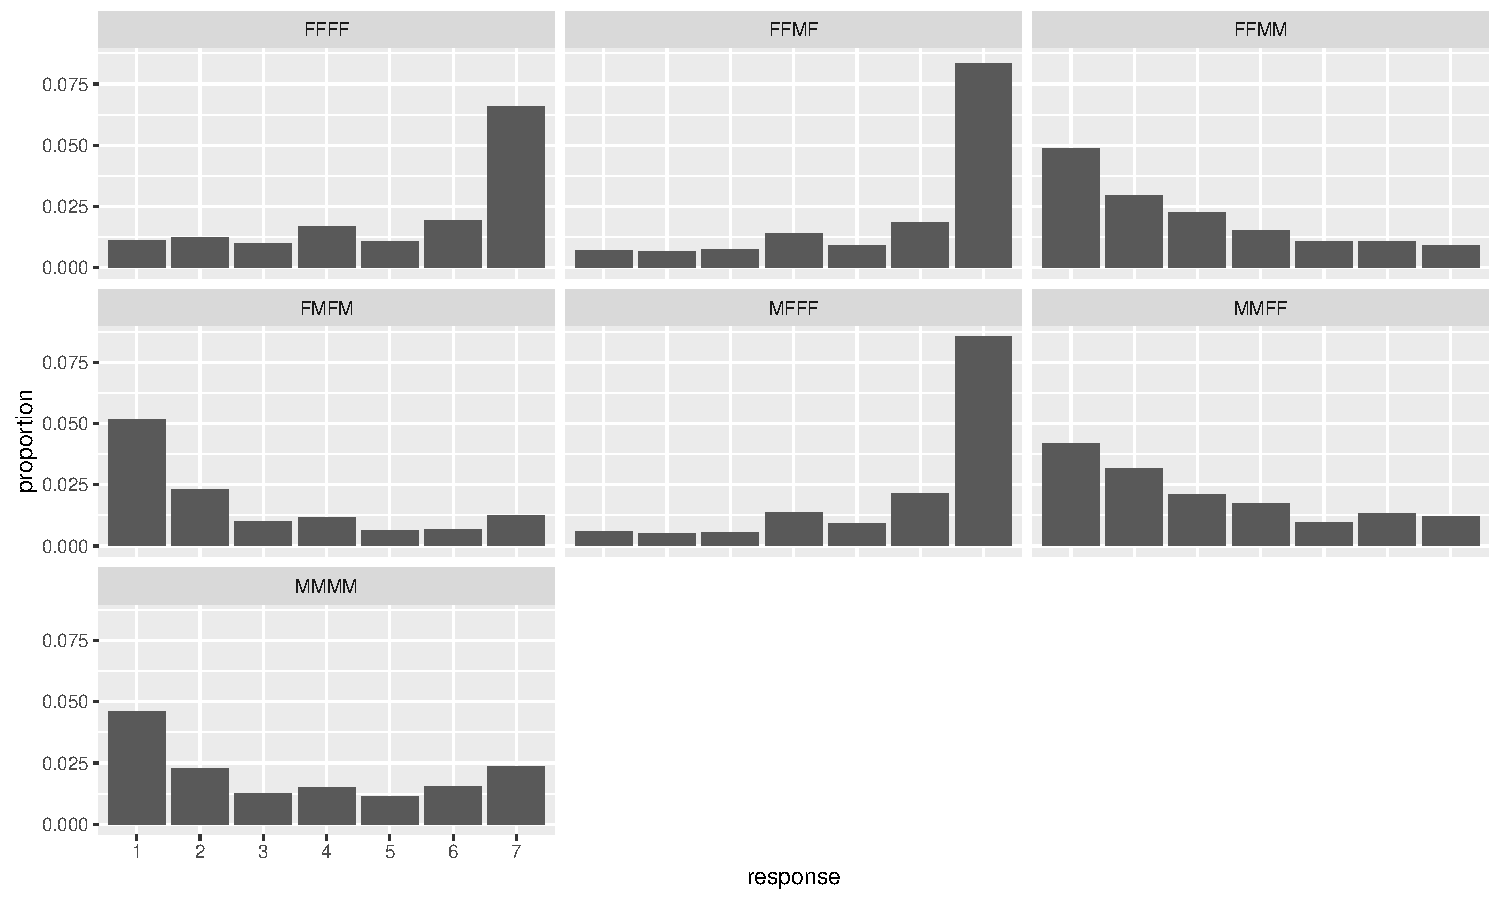
\includegraphics[height=.35\textheight]{figures/14mmmm-resps-1.pdf}
		\caption{All responses by all participants.}\label{14:fig:all-resps}
	\end{figure}


% \newpage

\begin{figure}[b]
	\centering
	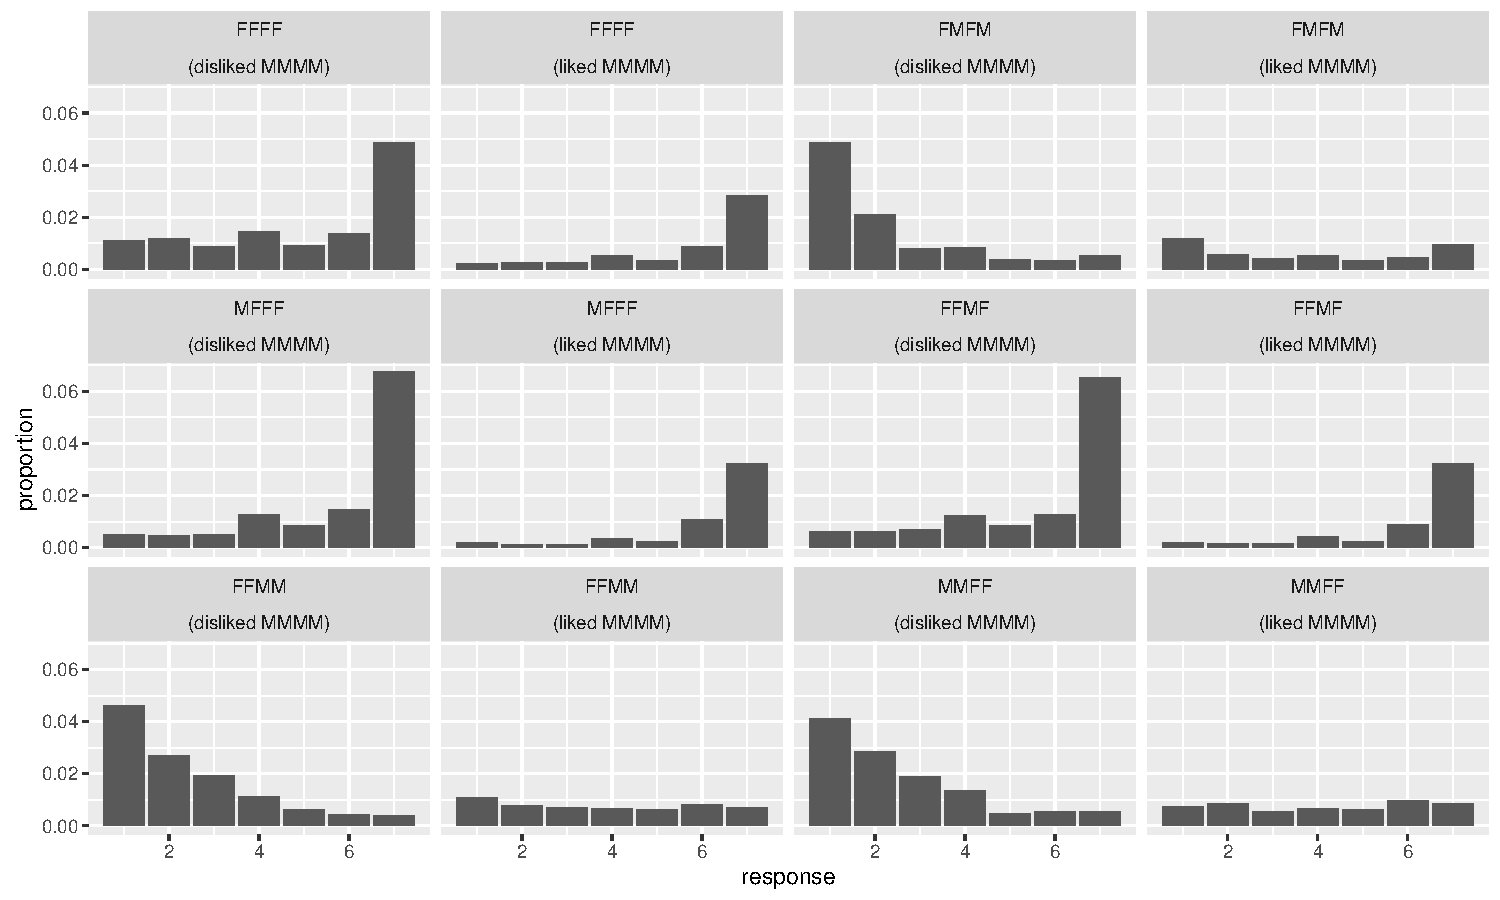
\includegraphics[height=.35\textheight]{figures/14all-resps.pdf}
	\caption{All responses by all participants according to whether the speaker liked or disliked the sentences in the \textsc{mmmm} condition.}\label{14:fig:all-resps-mmmm}
\end{figure}

\figref{14:fig:all-resps} shows the distribution of responses under each condition from all participants for the baselines (first column) and our four experimental conditions (second and third column). The baselines show strong grammaticality effects: feminine agreement with feminine subjects was rated as grammatical, while masculine agreement was unacceptable. A u-shaped
type of distribution for \textsc{mmmm} (masculine agreement with masculine subjects) suggests that although the majority of
speakers dispreferred it, some speakers clearly did find it grammatical. With mismatching subjects, feminine agreement (\textsc{ffmf} and \textsc{mfff}) was rated as grammatical, as shown in the second column. More gradient (un)acceptability was found for  \textsc{ffmm} and \textsc{mmff} (third column).

We compared the responses for all conditions based on whether speakers liked the \textsc{mmmm} combination (median rating $\geq$ 4) or disliked it (\figref{14:fig:all-resps-mmmm}). In total, 51 speakers found the \textsc{mmmm} combination grammatical. The overall picture shows that the distributions concerning the grammatical patterns are fundamentally the same, regardless of whether the speaker liked \textsc{mmmm} or not (the first two rows). However, there was in fact a difference for conditions with low acceptability scores (\textsc{ffmm} and \textsc{mmff}), as it can be seen in the final row of \figref{14:fig:all-resps-mmmm}. Speakers who liked \textsc{mmmm} showed no clear preference or dispreference for either of the mismatching combinations -- they were perceived as equally bad.

\begin{figure}[b]
	\centering
	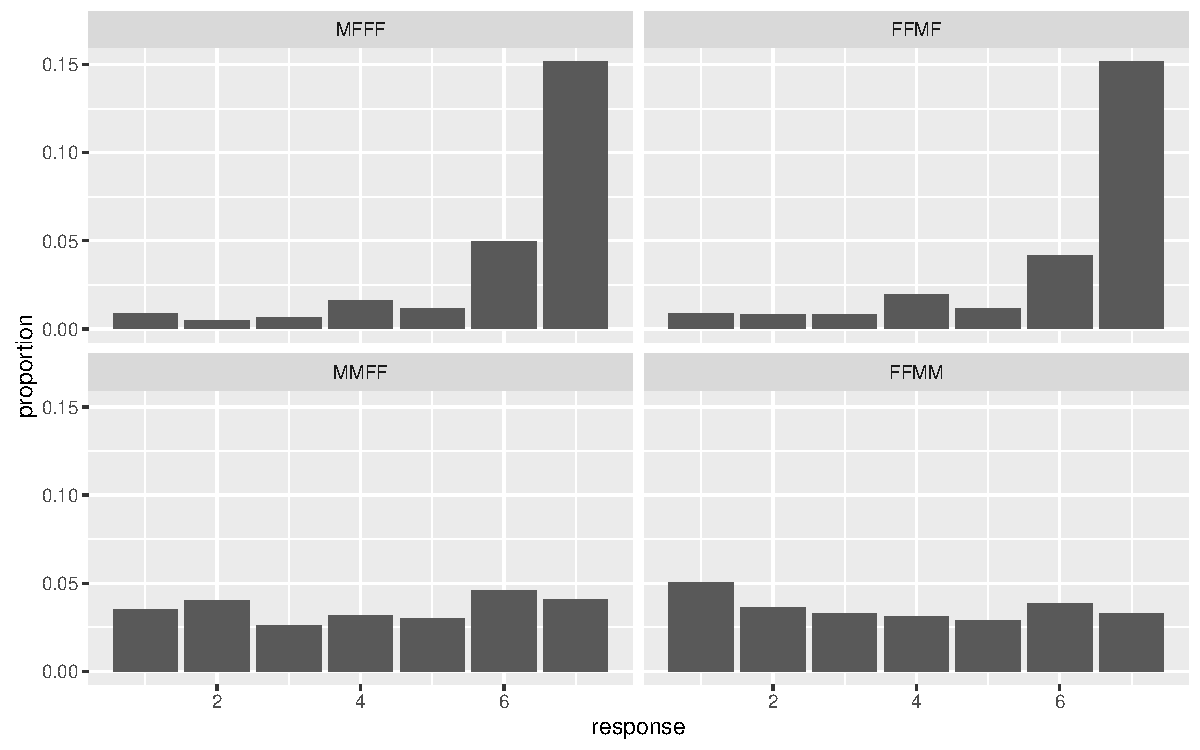
\includegraphics[height=.35\textheight]{figures/14resps-final.pdf}
	\caption{Responses by participants who liked \textsc{mmmm} \mbox{(median rating $\geq$ 4)\hspace*{-6mm}}}\label{14:fig:resps-final}
\end{figure}

\figref{14:fig:resps-final} shows the four crucial conditions just for those speakers who rated the \textsc{mmmm} baseline higher than 4. We see that the patterns with feminine agreement throughout were overwhelmingly acceptable and grammatical to these speakers, while the conditions with mismatches show more variation and received comparably lower scores.

To clarify whether the differences in these responses  were statistically significant, we fitted an ordinal regression model with only \texttt{condition} as a dependent variable, and \texttt{participant} and \texttt{hybrid\_noun} as random effects (see the Appendix for further details about the model).\footnote{Ordinal regression assumes an ordered discrete response variable. This is exactly the kind of data one obtains from grammaticality judgement tasks. In the models, \texttt{gender} and \texttt{region} did not play a role.}		
 
 
As the plot in \figref{14:fig:postmeans} shows, the factors with overlapping confidence intervals are not statistically different from each other. 
 We see that \textsc{ffmf} and \textsc{mfff} slightly overlap with 0, which means that they are not statistically different from the intercept (the grammatical baseline \textsc{ffff}). 		
On the other hand, \textsc{ffmm} and \textsc{mmff} are statistically worse than the intercept, but not different from each other or the ungrammatical baseline \textsc{fmfm}.%\largerpage[3]

\begin{figure}[h]
	\centering
	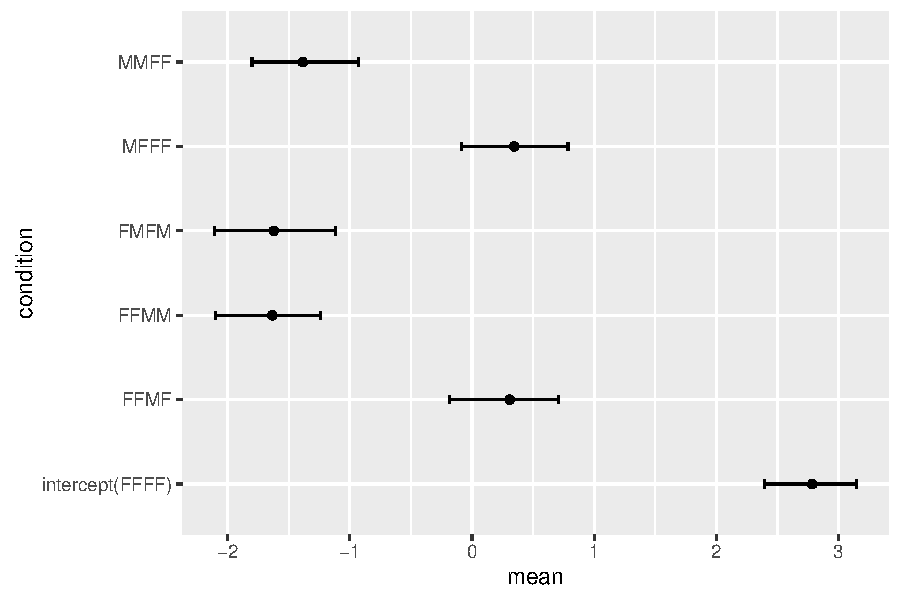
\includegraphics[height=.35\textheight]{figures/14model-plot.pdf}
	\caption{Posterior means and 95\% confidence intervals for the Bayesian regression model.}
	\label{14:fig:postmeans}
\end{figure}

The conclusion we can draw from this is that gender mismatches are possible in either direction as long as the adjectival agreement is feminine. 
 This is shown in \REF{14:ex17} and \REF{14:ex18}.



 \ea \textbf{Two-way mismatches possible with feminine agreement}\label{14:ex17}
\ea[]{\gll Jovan je redovn{-a} mušterija, a Milica povremen{-a} $\langle$\hspace{-2pt} mušterija$\rangle$.\\
  		Jovan is regular{-\textsc{f}} customer and Milica occasional{-\textsc{f}} {} customer\\
  		\glt `Jovan is a regular customer and Milica an occasional one.'\hfill  \textsc{mfff}}
\ex[]{\gll Milica je povremen{-a} mušterija, a Jovan redovn{-a} $\langle$\hspace{-2pt} mušterija$\rangle$.\\
  		Milica is occasional{-\textsc{f}} customer and Jovan regular{-\textsc{f}} {} customer\\
  		\glt `Milica is an occasional customer and Jovan a regular one.'\hfill  \textsc{ffmf}}
        \z \z
  		
\ea \textbf{No mismatch possible with masculine agreement}\label{14:ex18}
\ea[*]{\gll Milica je povremen{-a} mušterija, a Jovan redovn{-i} $\langle$\hspace{-2pt} mušterija$\rangle$.\\
  		Milica is occasional{-\textsc{f}} customer and Jovan regular{-\textsc{m}} {} customer\\
  		\glt `Milica is an occasional customer and Jovan a regular one.'\hfill  \textsc{ffmm}}
\ex[*]{\gll Jovan je redovn{-i} mušterija, a Milica povremen{-a} $\langle$\hspace{-2pt} mušterija$\rangle$.\\
  		Jovan is regular{-\textsc{m}} customer and Milica occasional{-\textsc{f}} {} customer\\
  		\glt `Jovan is a regular customer and Milica an occasional one.'\hfill  \textsc{mmff}}
        \z \z

\noindent Thus, with regard to the noun classes in \tabref{14:t2}, our hybrid nouns behave like nouns of the two-way alternating \textit{actor}-class when there is agreement in grammatical gender (feminine), but they behave like non-alternating nouns of the \textit{brother}-class if at least one of them bears natural gender (masculine).
		
		
\section{Analysis}	
		
		First, let us assume that the identity requirement for elided material involves \citeauthor{merchant2001}'s (\citeyear{merchant2001}) e-\textsc{given}ness (i.e. mutual entailment), as defined in \REF{14:egive}, where existential ($\exists$)-type shifting is ``a type-shifting operation that raises the expressions of type $t$ and existentially binds unfilled arguments'' while F-closure of $\alpha$ ``is the result of replacing F-marked parts of $\alpha$ with $\exists$-bound variables of the appropriate type (modulo $\exists$-type shifting)'' \citep[14]{merchant2001}: 
		
		\ea \label{14:egive} \textbf{e-\textsc{given}ness} \citep[26]{merchant2001}\\
		An expression E counts as e-\textsc{given} iff E has a salient antecedent A and, modulo $\exists$-type shifting,
        \begin{xlist}
		\exi{(i)}{A entails F-clo(E), and}
		\exi{(ii)}{E entails F-clo(A).}
        \end{xlist}
        \z

     
\newpage      
\noindent This condition requires that mutual entailment holds between the antecedent and the ellipsis site. This prevents semantically-equivalent, non-matching ellipsis sites \REF{14:ex20b} \citet[27]{merchant2001}.
		
		\ea
		\ea[]{Abby \textit{called Ben an idiot} after Mary did $\langle$call Ben an idiot$\rangle$. \\
		($\exists x\semdot x$ called Ben an idiot${}\leftrightarrow \exists x\semdot x$ called Ben an idiot)}\label{14:ex20a}
		\ex[\#]{Abby \textit{called Ben an idiot} after Mary did $\langle$insult Ben$\rangle$. \\
		($\exists x\semdot x$ called Ben an idiot $\nleftrightarrow \exists x\semdot x$ insulted Ben)}\label{14:ex20b}
        \z \z
        
\noindent Following \citet{cooper83}, it is often assumed that (natural) gender features can introduce presuppositions \citep[also see][]{sauerland03,sauerland08,heim08,kratzer09,spathas10,sudo-diss}.
		In Greek, non-alternating nouns of the \textit{brother}-class have been claimed to contain a presupposition about gender of the referent \REF{14:ex21} (\citealt[19]{merchant14}, \citealt[715]{sudospathas-sub20}).
		
		\ea \label{14:ex21}
		\ea \evalfun{adherfos}${}=\lambda x_e : \textsc{male}(x)\semdot \textsc{sibling}(x)$
		\ex \evalfun{adherfi}${}=\lambda x_e : \textsc{female}(x)\semdot \textsc{sibling}(x)$	         
        \z \z
        

\ea 
		\ea[*]{\gll O Petros ine kalos adherfos, ala i Maria ine mia kakia\hspace{33pt} $\langle$\hspace{-2pt} adherfi$\rangle$.\\
		the Petros is good.\textsc{m} brother but the Maria is a.\textsc{f} bad.\textsc{f} {} sister\\
		\glt Intended: `Petros is a good brother, but Maria is a bad one (sister).'}
		\ex[*]{\gll I Maria ine kali adherfi, ala o Petros ine enes kakos\hspace{38pt} $\langle$\hspace{-2pt} adherfos$\rangle$.\\
		the Maria is good.\textsc{f} sister but the Petros is a.\textsc{m} bad.\textsc{m} {} brother\\
		\glt Intended: `Petros is a good brother, but Maria is a bad one (sister).'	 \\ \hspace*\fill (Greek; \citealt[12]{merchant14})}
        \z \z
		
\noindent The elided and antecedent noun have conflicting gender presuppositions, not mutually-entailing:	
		
		\ea $\exists x: \textsc{male}(x)\semdot \textsc{sibling}(x)\nleftrightarrow \exists x: \textsc{female}(x)\semdot \textsc{sibling}(x)$
        \z
		
\noindent		In the analysis of two-way alternating  ``epicene'' nouns, however, it is often assumed that they do not contain any lexical presuppositions 
		about gender \REF{14:ex24}, and thus ellipsis is licensed \REF{14:doctor}.
		
		\ea \evalfun{jatros}${}=\lambda x_e\semdot \textsc{doctor}(x)$	\label{14:ex24}
        \z
        
\ea 
		\ea \gll O Petros ine kalos jatros, ala i Maria ine mia kakia $\langle$\hspace{-2pt} jatros$\rangle$.\\	 
		the Petros is good.\textsc{m} doctor but the Maria is a.\textsc{f} bad.\textsc{f} {} doctor\\
		\glt `Petros is a good doctor, but Maria is a bad one.'
		\ex \gll I Maria ine kali jatros, ala o Petros ine enas kakos $\langle$\hspace{-2pt} jatros$\rangle$.\\	 
		the Maria is good.\textsc{f} doctor but the Petros is a.\textsc{m} bad.\textsc{m} {} doctor\\
		`Maria is a good doctor, but Petros is a bad one.'	 \\ \hspace*\fill (Greek; \citealt[15]{merchant14})	
        \z \z
		
		\ea\label{14:doctor} $\exists x\semdot \textsc{doctor}(x)\leftrightarrow \exists x\semdot \textsc{doctor}(x)$        
        \z
        
\noindent If we adopt a similar approach for hybrid nouns in BCS, then hybrid nouns agreeing in grammatical gender (feminine) do not contain any presupposition about gender, while the hybrid nouns that agree in natural gender (masculine) should have an additional gender presupposition. Assuming that the grammatical feminine gender of hybrid nouns does not contribute any gender presupposition, this would make it compatible with male and female referents:
		
		\ea \evalfun{$n$\sub{[\textsc{f}]}}${}=\lambda P\lambda x\semdot P(x)$ \z
		
\noindent		For masculine-agreeing hybrid nouns, let us assume that the denotation of natural gender is a partial identity function restricting the set of customers to the set of male customers \citep{cooper83}.
		
		\ea \evalfun{$n$\sub{[\textsc{m}]}}${}= \lambda P\lambda x: \textsc{male}(x)\semdot P(x)$
        \z


\noindent The introduction of a gender presupposition with masculine agreeing hybrid nouns makes them incompatible with female referents.\footnote{While other theories rule out such examples based on competition with the feminine agreeing form (e.g. Maximize Presupposition; \citealt[148f.]{bobaljikzocca} or  Principle of Gender Competition; \citealt[722]{sudospathas-sub20}), we argue that the syntactic presence of both features is necessary based on instances of mixed agreement, such as  \REF{14:mismatchbcs}.}
		
% 		\begin{multicols}{2}
			
			\ea \ea[]{\gll Marija nam je nov-a mušterija. \label{14:exa}\\
			Marija us is new-\textsc{f} customer\\
			\glt `Marija is our new customer.'}
			\ex[*]{\gll Marija nam je nov-i mušterija. \label{14:exb}\\
			Marija us is new-\textsc{m} customer\\
			\glt `Marija is our new customer.'}
            \z \z
			
% 		\end{multicols}	

\newpage 
		\ea \evalfun{novi mušterija}${}=\lambda x\semdot \textsc{customer}(x)$, defined only if $x$ is male
		\ea \evalfun{\REF{14:exa}}${}=\textsc{customer}(\textsc{Marija})$
		\ex \evalfun{\REF{14:exb}}${}=\textsc{customer}(\textsc{Marija})$, defined only if Marija is male\\\hspace*\fill\textit{(presupposition failure!)}
        \z \z


\noindent Returning to gender mismatches under ellipsis, in an example such as \REF{14:ex31}, involving feminine agreement in both clauses, both instances of \textit{mušterija} will lack natural gender feature and the corresponding presupposition.
		
		\ea\gll Milica je povremen{-a} mušterija, a Jovan redovn{-a} $\langle$\hspace{-2pt} mušterija$\rangle$.\\
		Milica is occasional{-\textsc{f}} customer and Jovan regular{-\textsc{f}} {} customer\\
		\glt `Milica is an occasional customer and Jovan a regular one.'\hfill  \textsc{ffmf}\label{14:ex31}
        \z
		
\noindent		In order to analyze the ellipsis patterns, we adopt the assumptions of Distributed Morphology that nouns are built up from a category neutral root and a head $n$ that categorizes this root as nominal \citep{hallemarantz93,harleynoyer99,kihm05,acquaviva09,kramerbook}. Following \citet{kramerbook}, we will treat gender for now as a feature introduced by $n$ (although see below for more detail about the different possibilities of simultaneous separate structural encoding of natural and grammatical gender on hybrid nouns). We assume further that number features of nouns are introduced on a NumP. These assumptions yield the structure for \REF{14:ex31} as given in \REF{14:ex32}, where ellipsis is triggered by an [E] feature on Num \citep[e.g.][]{merchant14,saabliptak16,saab-nomel}. 		


 		\setlength{\columnsep}{-3.5em}     
\begin{multicols}{2}		
			
			\ea \textbf{Antecedent}:\label{14:ex32}\vspace{6pt}\\		
			\leavevmode\vadjust{\vspace{-\baselineskip}}\newline
			\begin{tikzpicture}[>=latex',scale=0.85]
			\tikzset{every tree node/.style={align=center,anchor=north}}
			\Tree [.DP D [.... \node(a){A\\{povremen-a}}; [.NumP Num
			[.\node(np){$n$P}; 
			\node(n){$n$\\{\footnotesize [\textsc{f}]}}; \node(root){$\sqrt{\text{mušterija}}$}; ]]]]
			\node[draw,rounded corners,fit=(np)(n)(root)]{};
			%\draw[semithick,->,dashed,rounded corners] (a.south) -- ++(0,-7.5em)coordinate (x) -- ($(x-|n)$) -- (n.south);
			\end{tikzpicture}
            \z
			
			\columnbreak
			
			\begin{exe}
            \exi{}{\textbf{Ellipsis site}:\vspace{6pt}\\		
			\leavevmode\vadjust{\vspace{-\baselineskip}}\newline
			\begin{tikzpicture}[>=latex',scale=0.85]
			\tikzset{every tree node/.style={align=center,anchor=north}}
			\Tree [.DP D [.... \node(a){A\\{redovn-a}}; [.NumP Num\sub{[E]} 
			[.\node(np){$n$P}; 
			\node(n){$n$\\{\footnotesize [\textsc{f}]}}; \node(root){$\sqrt{\text{mušterija}}$}; ]]]]
			\node[draw,rounded corners,dashed,fit=(np)(n)(root)]{};
			\draw[semithick,->,dashed,rounded corners] (a.south) -- ++(0,-7.5em)coordinate (x) -- ($(x-|n)$) -- (n.south);
			\end{tikzpicture}  }
	\end{exe}	
	\end{multicols} 
    
        
\noindent Importantly, from the point of view of the e-\textsc{given}ness condition in \REF{14:egive},  mutual entailment  is trivially satisfied  since the elided material is identical.
		
		\ea
		\leavevmode\vadjust{\vspace{-\baselineskip}}\newline
		\begin{tabular}{ccc}
			\evalfun{\begin{tikzpicture}[baseline=(current bounding box.center)] 
				\tikzset{every tree node/.style={align=center,anchor=north}} \Tree [.\node(np){$n$P}; 
				\node(n){$n$\\{\footnotesize [\textsc{f}]}}; \node(root){$\sqrt{\text{mušterija}}$}; ]
				\end{tikzpicture}}
			& {\Large $\leftrightarrow$ }  &
			\evalfun{\begin{tikzpicture}[baseline=(current bounding box.center)] 
				\tikzset{every tree node/.style={align=center,anchor=north}} \Tree [.\node(np){$n$P}; 
				\node(n){$n$\\{\footnotesize [\textsc{f}]}}; \node(root){$\sqrt{\text{mušterija}}$}; ]
				\end{tikzpicture}}\smallskip\\
			$\exists x\semdot \textsc{customer}(x)$ & & $\exists x\semdot \textsc{customer}(x)$\\
		\end{tabular} 
        \z
		
        
\noindent However, as soon as we have masculine agreement on one of the conjuncts, we necessarily have the relevant natural gender feature  [\textsc{m}] of the referent, making the ellipsis unacceptable \REF{14:ex34}. The relevant structure, demonstrating the lack of feature identity, is given in \REF{14:ex35}.
		
		\ea[*]{\gll Milica je povremen{-a} mušterija, a Jovan redovn{-i} $\langle$\hspace{-2pt} mušterija$\rangle$.\\
		Milica is occasional{-\textsc{f}} customer and Jovan regular{-\textsc{m}} {} customer\\
		\glt `Milica is an occasional customer and Jovan a regular one.'\hfill  \textsc{ffmm}}\label{14:ex34}
        \z
		
%  \newpage		
		\begin{multicols}{2}		
			
			\ea \textbf{Antecedent}:\label{14:ex35}\vspace{6pt}\\		
			\leavevmode\vadjust{\vspace{-\baselineskip}}\newline
			\begin{tikzpicture}[>=latex',scale=0.85]
			\tikzset{every tree node/.style={align=center,anchor=north}}
			\Tree [.DP D [.... \node(a){A\\{povremen-a}}; [.NumP Num 
			[.\node(np){$n$P}; 
			\node(n){$n$\\{\footnotesize [\textsc{f}]}}; \node(root){$\sqrt{\text{mušteria}}$}; ]]]]
			\node[draw,rounded corners,fit=(np)(n)(root)]{};
			%\draw[semithick,->,dashed,rounded corners] (a.south) -- ++(0,-7.5em)coordinate (x) -- ($(x-|n)$) -- (n.south);
			\end{tikzpicture}  
            \z
			
			\columnbreak
			
			\begin{exe}
            \exi{}{\textbf{Ellipsis site}:\vspace{6pt}\\		
			\leavevmode\vadjust{\vspace{-\baselineskip}}\newline
			\begin{tikzpicture}[>=latex',scale=0.85]
			\tikzset{every tree node/.style={align=center,anchor=north}}
			\Tree [.DP D [.... \node(a){A\\{redovn-i}}; [.NumP Num\sub{[E]}  
			[.\node(np){$n$P}; 
			\node(n){$n$\\{\footnotesize [\textsc{m}]}}; \node(root){$\sqrt{\text{mušterija}}$}; ]]]]]
			\node[draw,rounded corners,dashed,fit=(np)(n)(root)]{};
			\draw[semithick,->,dashed,rounded corners] (a.south) -- ++(0,-7.5em)coordinate (x) -- ($(x-|n)$) -- (n.south);
			\end{tikzpicture}  }
            \end{exe}
			
		\end{multicols}
        
\noindent Recall that the masculine feature also introduces the presupposition that the referent is male. If there is no corresponding feature in the antecedent, then e-\textsc{given}ness is violated because there being a customer does not entail there being a male customer:
		
		\ea 
		\leavevmode\vadjust{\vspace{-\baselineskip}}\newline
		\begin{tabular}{ccc}
			\evalfun{\begin{tikzpicture}[baseline=(current bounding box.center)] 
				\tikzset{every tree node/.style={align=center,anchor=north}} \Tree [.\node(np){$n$P}; 
				\node(n){$n$\\{\footnotesize [\textsc{f}]}}; \node(root){$\sqrt{\text{mušterija}}$}; ]
				\end{tikzpicture}}
			& {\Large $\nrightarrow$ }  &
			\evalfun{\begin{tikzpicture}[baseline=(current bounding box.center)] 
				\tikzset{every tree node/.style={align=center,anchor=north}} \Tree [.\node(np){$n$P}; 
				\node(n){$n$\\{\footnotesize [\textsc{m}]}}; \node(root){$\sqrt{\text{mušterija}}$}; ]
				\end{tikzpicture}}\smallskip\\
			$\exists x\semdot \textsc{customer}(x)$ & & $\exists  x: \textsc{male}(x)\semdot \textsc{customer}(x)$\\
		\end{tabular}  \z
			
\noindent		The same situation holds if masculine agreement obtains in the antecedent:
		
		\ea[*]{\gll Jovan je redovn{-i} mušterija, a Milica povremen{-a} $\langle$\hspace{-2pt} mušterija$\rangle$.\\
		Jovan is regular{-\textsc{m}} customer but Milica occasional{-\textsc{f}} {} customer\\
		`Jovan is a regular customer and Milica an occasional one.'\hfill  \textsc{mmff}}\label{14:ex37}	
        \z
		
        
\noindent Since \textit{mutual} entailment is required, the existence of masculine gender at only one of the conjuncts results in ungrammaticality, since the e-\textsc{given}ness requirement is not met.\largerpage[2]
		
		\ea 
		\leavevmode\vadjust{\vspace{-\baselineskip}}\newline
		\begin{tabular}{ccc}
			\evalfun{\begin{tikzpicture}[baseline=(current bounding box.center)] 
				\tikzset{every tree node/.style={align=center,anchor=north}} \Tree [.\node(np){$n$P}; 
				\node(n){$n$\\{\footnotesize [\textsc{m}]}}; \node(root){$\sqrt{\text{mušterija}}$}; ]
				\end{tikzpicture}} & {\Large $\nleftarrow$ }  &
			\evalfun{\begin{tikzpicture}[baseline=(current bounding box.center)] 
				\tikzset{every tree node/.style={align=center,anchor=north}} \Tree [.\node(np){$n$P}; 
				\node(n){$n$\\{\footnotesize [\textsc{f}]}}; \node(root){$\sqrt{\text{mušterija}}$}; ]
				\end{tikzpicture}}\smallskip\\
			$\exists x: \textsc{male}(x)\semdot\textsc{customer}(x)$ & & $\exists x\semdot\textsc{customer}(x)$ \\
		\end{tabular}  \z
		
\noindent		This accounts for why mismatches in referent gender are not tolerated if the adjective agrees in masculine in one conjunct only.
		As we expect, if we have two masculine referents \REF{14:refmmmm}, then mutual entailment is restored \REF{14:ex40}. 
		
		\ea\gll Uroš je redovn{-i} mušterija, a Tomislav povremen{-i} $\langle$\hspace{-2pt} mušterija$\rangle$. \label{14:refmmmm}\\
		Uroš is regular{-\textsc{m}} customer and Tomislav occasional{-\textsc{m}} {} customer\\
		\glt `Uroš is a regular customer and Tomislav an occasional one.'\hfill  \textsc{mmmm} 	
        \z
		
		\ea \label{14:ex40}
		\leavevmode\vadjust{\vspace{-\baselineskip}}\newline
		\begin{tabular}{ccc}
			\evalfun{\begin{tikzpicture}[baseline=(current bounding box.center)] 
				\tikzset{every tree node/.style={align=center,anchor=north}} \Tree [.\node(np){$n$P}; 
				\node(n){$n$\\{\footnotesize [\textsc{m}]}}; \node(root){$\sqrt{\text{mušterija}}$}; ]
				\end{tikzpicture}} & {\Large $\leftrightarrow$ }  &
			\evalfun{\begin{tikzpicture}[baseline=(current bounding box.center)] 
				\tikzset{every tree node/.style={align=center,anchor=north}} \Tree [.\node(np){$n$P}; 
				\node(n){$n$\\{\footnotesize [\textsc{m}]}}; \node(root){$\sqrt{\text{mušterija}}$}; ]
				\end{tikzpicture}}  \smallskip\\
			$\exists x : \textsc{male}(x)\semdot \textsc{customer}(x)$ & &  $\exists x: \textsc{male}(x)\semdot \textsc{customer}(x)$ \\
		\end{tabular}  	\z
		
\noindent		Exactly why masculine agreement with hybrid nouns \REF{14:refmmmm} is not possible for all speakers is an open issue, and we suggest it could be due to not all speakers having the variant of $n$ containing the additional [\textsc{m}] feature. We leave further examination of interspeaker variation to future research.	

\subsection{The encoding of natural and grammatical gender features}
		
Since the nouns addressed in this paper have the possibility to simultaneously encode both the grammatical feminine and the natural masculine gender (as illustrated by \REF{14:mismatchbcs}, see also \citealt{wandz03,despichybrid17,puskar17}), a question that remains open is where exactly these features are encoded in the DP structure.		
  
Some accounts \citep{matushansky13,pesetsky14,Landau2016DPinternalsemantic} assume grammatical gender to be encoded low in the noun's structure, as a property related to the nominal stem. Natural gender is optionally introduced on a higher functional projection. Under this approach, we would treat the grammatical feminine gender of our hybrid nouns as a property of $n$, while natural gender would be introduced at a higher functional projection (e.g. GenP, \citealt[cf.][]{picallo91}). The lower gender would not introduce any gender presuppositions, while the denotation of the gender on Gen would be a partial identity function restricting the set of customers to the set of male customers \citep{cooper83}. If the male-referring hybrid noun triggers feminine agreement, adjectival concord then targets the grammatical gender feature on $n$ \REF{14:ex41}.

%   \newpage
\ea\label{14:ex41}
		\leavevmode\vadjust{\vspace{-\baselineskip}}\newline
		\begin{tikzpicture}[>=latex']
		\tikzset{every tree node/.style={align=center,anchor=north}}
		\Tree  [.... \node(a){A\\{redovn-a}\\{\footnotesize [\textsc{f}]}}; [.\node[label={right:\footnotesize $\lambda x\semdot\textsc{customer}(x)$ }]{$n$P}; 
		\node(n){$n$\\{-a}\\{\footnotesize [\textsc{f}]}}; {$\sqrt{\text{mušterij-}}$} ]]
		\draw[semithick,->,dashed,rounded corners] (a.south) -- ++(0,-3.5em)coordinate (x) -- ($(x-|n)$) -- (n.south);
		\end{tikzpicture}    \z
        
        
\noindent For masculine-agreeing hybrid nouns, the closest target for Agree will be the higher masculine gender \REF{14:ex42}. %under the assumption that 
		
		\ea \label{14:ex42}
		\leavevmode\vadjust{\vspace{-\baselineskip}}\newline
		\begin{tikzpicture}[>=latex']
		\tikzset{every tree node/.style={align=center,anchor=north}}
		\Tree [.... \node(a){A\\{nov-i}\\{\footnotesize [\textsc{m}]}}; [.\node[label={right:\footnotesize $\lambda x: \textsc{male}(x)\semdot \textsc{customer}(x)$ }]{GenP}; 
		\node(gen){Gen\\{\footnotesize $\lambda P\lambda x: \textsc{male}(x)\semdot P(x)$}\\{\footnotesize [\textsc{m}]}}; 
		[.\node[label={right:\footnotesize $\lambda x\semdot\textsc{customer}(x)$ }]{$n$P}; 
		$n$\\{-a}\\{\footnotesize [\textsc{f}]} {$\sqrt{\text{mušterij-}}$} ]]]
		\draw[semithick,->,dashed,rounded corners] (a.south) -- ++(0,-3.5em)coordinate (x) -- ($(x-|gen)$) -- (gen.south);
		%\node[right of=gen,xshift=2em] {\footnotesize $\lambda$P.$\lambda{}x$: $x$ is male. P($x$)};
		\end{tikzpicture} \\
		\begin{tabular}{lll}
			&&\\
			\evalfun{$n$P} & $=$ & $\lambda x\semdot\textsc{customer}(x)$ \\
			&&\\
			\evalfun{GenP} & $=$ & \evalfun{Gen}(\evalfun{$n$P}) \smallskip\\
			& $=$ & $[\lambda P\lambda x:\textsc{male}(x)\semdot P(x)](\lambda x\semdot\textsc{customer}(x))$\smallskip\\
			& $=$ & $\lambda x :\textsc{male}(x)\semdot [\lambda x'\semdot\textsc{customer}(x')](x)$ \smallskip\\
			& $=$ & $\lambda x :\textsc{male}(x)\semdot \textsc{customer}(x)$\\
			\end{tabular} \z
			

\noindent Ellipsis would be licensed if neither the antecendent nor the elided noun project the GenP, or if both of them do. The existence of GenP and the masculine feature in either the antecedent or the ellipsis site would lead to a lack of mutual entailment and the concomitant impossibility of ellipsis, in the manner proposed above.
			
			Another theoretical option would be to make the GenP the locus of grammatical gender, and the $n$ of the natural one for the hybrid nouns of this particular type (see \citealt{puskar17,puskarhybrid17}). A hybrid noun with no natural gender would be represented as \REF{14:ex43}, while the noun with the natural gender feature would have the structure in \REF{14:ex44}. Under this approach, the natural gender feature of $n$ would have a more complex syntactic representation than the grammatical one. The gender probe is relativized towards the more complex gender. If this gender is present on the $n$, it will be the preferred goal for Agree \REF{14:ex44}. If it is absent, Agree would copy the higher grammatical gender \REF{14:ex43} (see \citealt{puskar17} for further detail).  
			
			\begin{multicols}{2}
			\ea \label{14:ex43} 
			\leavevmode\vadjust{\vspace{-\baselineskip}}\newline
			\begin{tikzpicture}[>=latex']
			\tikzset{every tree node/.style={align=center,anchor=north}}
			\Tree [.... \node(a){A\\{nov-a}\\{\footnotesize [\textsc{f}]}}; [.\node{GenP}; 
			\node(gen){Gen\\{-a}\\{\footnotesize [\textsc{f}]}}; 
			[.\node{$n$P}; 
			$n$ {$\sqrt{\text{mušterij-}}$} ]]]
			\draw[semithick,->,dashed,rounded corners] (a.south) -- ++(0,-3.5em)coordinate (x) -- ($(x-|gen)$) -- (gen.south);
			%\node[right of=gen,xshift=2em] {\footnotesize $\lambda$P.$\lambda{}x$: $x$ is male. P($x$)};
			\end{tikzpicture} \\ \z
			
			\columnbreak
			\ea\label{14:ex44}
			\leavevmode\vadjust{\vspace{-\baselineskip}}\newline
			\begin{tikzpicture}[>=latex']
			\tikzset{every tree node/.style={align=center,anchor=north}}
			\Tree [.... \node(a){A\\{nov-i}\\{\footnotesize [\textsc{m}]}}; [.\node{GenP}; 
			\node(gen){Gen\\{-a}\\{\footnotesize [\textsc{f}]}}; 
			[.\node{$n$P}; 
			\node(n){$n$\\{\footnotesize [\textsc{m}]}}; {$\sqrt{\text{mušterij-}}$} ]]]
			\draw[semithick,->,dashed,rounded corners] (a.south) -- ++(0,-5em)coordinate (x) -- ($(x-|n)$) -- (n.south);
			\end{tikzpicture} \\ \z
			
			\end{multicols}
    
\noindent If this analysis were to be adopted, the ungrammatical sentences would be ruled out by prohibiting  any mismatches between the features of antecedent and those of the ellipsis site (cf. \citealt{merchant13}). 
			
			To sum up, both types of approaches to the structural position of gender features would in principle be compatible with the results of our experiment. Future research should then be tasked with teasing apart the two and defining the exact locus of the natural and grammatical gender features. However, what the results undoubtedly reveal is the necessity to represent the two types of features separately, as well as that they differ in quality, such that natural gender has an additional meaning component.   
			
			
			\section{Conclusion}	
			
			This paper has presented new experimental data from  NP ellipsis showing that hybrid nouns in BCS show a split behaviour with regard to gender ellipsis: if they agree in feminine gender, then mismatches in referent gender are permitted for either the antecedent or elided noun. However, masculine agreement in either conjunct blocks gender mismatches. We have linked this to the optional presence of a natural [\textsc{m}] gender feature which represents a target for adjectival concord and introduces a gender presupposition.
			It is this gender presupposition that destroys the mutual entailment relation required by \citeauthor{merchant2001}'s (\citeyear{merchant2001}) e-\textsc{given}ness requirement on ellipsis licensing.
			Consequently,  this study suggest that natural masculine gender is syntactically absent when the adjective agrees in grammatical gender.
		
		
    
    
\section*{Abbreviations}

\begin{tabularx}{.5\textwidth}{@{}lQ@{}}
\textsc{f}&feminine\\
\textsc{m}&masculine\\
\textsc{pl}&plural\\
\end{tabularx}%
\begin{tabularx}{.5\textwidth}{@{}lQ@{}}
\textsc{refl}&reflexive\\
\textsc{sg}&singular\\
&\\
\end{tabularx}



\section*{Acknowledgements}

We would like to thank Ana Bosni\'{c} and Joanna Zaleska for the help with the experimental design and coding, as well as Boban Arsenijevi\'{c}, Jelena Stojkovi\'{c}, Andrew Nevins and the audience of FDSL 12 for the valuable comments and feedback.   



\section*{Appendix}	
		
We use an ordinal Bayesian regression model with the package \texttt{MCMCglmm} \citep{Hadfield.2010} in R \citep{rcore}. We used non-informative priors (an inverse gamma with V=1 and nu=0.002).  Table \ref{14:tab:estimates} presents the posterior mean estimates, the confidence intervals and equivalent of a Bayesian p value. The corresponding posterior estimates of the random effects can be are shown in Table \ref{14:tab:random-estimates}.

\begin{table} 
\footnotesize

% \hspace*{-0.2em}\resizebox{.95\textwidth}{!}{
\begin{tabularx}{\textwidth}{lrrrrrr}
\lsptoprule
& post.mean & l-95\% CI & u-95\% CI & effect sample & pMCMC    &    \\
(Intercept)            & 2.7552    & 2.3839    & 3.1941    & 354.0         & $<$0.002 & ** \\
condition FFMF         & 0.3172    & $-$0.1073   & 0.7484    & 600.0         & 0.1433   &    \\
condition FFMM         & $-$1.6084   & $-$2.0599   & $-$1.2233   & 487.7         & $<$0.002 & ** \\
condition FMFM         & $-$1.6095   & $-$2.0645   & $-$1.0990   & 600.0         & $<$0.002 & ** \\
condition MFFF         & 0.3723    & $-$0.0990   & 0.7610    & 516.1         & 0.0933   & .  \\
condition MMFF         & $-$1.3541   & $-$1.8228   & $-$0.9690   & 514.2         & $<$0.002 & ** \\
\midrule
Cutpoints:                                                                                 \\
& post.mean & l-95\% CI & u-95\% CI & effect sample                 \\
cutpoint trait value.1 & 0.6284    & 0.5391    & 0.7129    & 90.48                         \\
cutpoint trait value.2 & 1.0485    & 0.9316    & 1.1437    & 62.66                         \\
cutpoint trait value.3 & 1.5598    & 1.4347    & 1.6683    & 30.25                         \\
cutpoint trait value.4 & 1.9236    & 1.8068    & 2.0575    & 29.95                         \\
cutpoint trait value.5 & 2.6803    & 2.5527    & 2.8159    & 43.93                         \\
\lspbottomrule
\end{tabularx}
% }
\caption{Coefficients for the MCMC model with confidence intervals and cutpoints.}
\label{14:tab:estimates}
\end{table}


\begin{table}[h]
\centering
\footnotesize
\begin{tabularx}{\textwidth}{lXXXX}
\lsptoprule
& post.mean & l-95\% CI & u-95\% CI & effect sample \\
participant & 0.3557    & 0.2037    & 0.512     & 478.8         \\
\midrule
& post.mean & l-95\% CI & u-95\% CI & effect sample \\
hybrid noun & 0.06491   & 0.004233  & 0.1571    & 600           \\
\lspbottomrule
\end{tabularx}
\caption{Random effects for the MCMC model.}\label{14:tab:random-estimates}
\end{table}		

{\sloppy
\printbibliography[heading=subbibliography,notkeyword=this]
}
\clearpage 
\end{document}
